\chapter{Systembeskrivelse}
	Systemet består af tre databaser via Firebase med brugeradgang via iOS og Android applikation.
	Databaserne indeholder brugere, projekter, PDF tegninger, information og objekter tilhørende projekterne.
	Et byggeprojekt indeholder en PDF tegning, tegne objekter, mulighed for upload af billede og tekst. \\
	
	\begin{figure}[H]
		\centering
		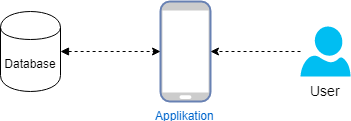
\includegraphics[width=0.4\linewidth]{Systembeskrivelse/Oversigtoversystem}
		\caption{Oversigt over systemet}
		\label{fig:OversigtSystembeskrivelse}
	\end{figure}
	
	Systemet skal kunne håndtere de byggeprojekter Rambøll har og oprette nye, når de overtager et nyt byggeprojekt.
	Disse skal kunne tilgåes af Rambølls ansatte, via enten en smartphone eller tablet.
	Rambølls ansatte får tildelt et personligt login for, at der kan holdes historik over, hvem der har oprettet projekter og registreringer.
	Brugere skal kunne oprette en registring for et givet projekt.
	Når en bruger er færdig med at oprette sin registrering, skal denne kunne eksporteres til en excel fil og sendes, som en vedhæftet fil i en mail.
	Systemet har en log, som indeholder en liste over alle registreringer til et givent projekt. \\	
				 
	\clearpage